\documentclass{beamer}
%Для защит онлайн лучше использовать разрешение 16x9
%\documentclass[aspectratio=169]{beamer}

%%% Обязательные пакеты
%% Beamer
\usepackage{beamerthemesplit}
\usetheme{SPbGU}
\beamertemplatenavigationsymbolsempty
\usepackage{appendixnumberbeamer}

%% Локализация
\usepackage{fontspec}
\setmainfont{CMU Serif}
\setsansfont{CMU Sans Serif}
\setmonofont{CMU Typewriter Text}
%\setmonofont{Fira Code}[Contextuals=Alternate,Scale=0.9]
%\setmonofont{Inconsolata}
% \newfontfamily\cyrillicfont{CMU Serif}

\usepackage{polyglossia}
\setdefaultlanguage{russian}
\setotherlanguage{english}

%% Графика
\usepackage{wrapfig} % Позволяет вставлять графику, обтекаемую текстом
\usepackage{pdfpages} % Позволяет вставлять многостраничные pdf документы в текст

%% Математика
\usepackage{amsmath, amsfonts, amssymb, amsthm, mathtools} % "Адекватная" работа с математикой в LaTeX

% Математические окружения с русским названием
\newtheorem{rutheorem}{Теорема}
\newtheorem{ruproof}{Доказательство}
\newtheorem{rudefinition}{Определение}
\newtheorem{rulemma}{Лемма}


%%% Дополнительные пакеты. Используются в презентации, но могут быть отключены при необходимости
\usepackage{tikz} % Мощный пакет для создание рисунков, однако может очень сильно замедлять компиляцию
\usetikzlibrary{decorations.pathreplacing,calc,shapes,positioning,tikzmark}

\usepackage{multirow} % Ячейка занимающая несколько строк в таблице

%% Пакеты для оформления алгоритмов на псевдокоде
\usepackage[noend]{algpseudocode}
\usepackage{algorithm}
\usepackage{algorithmicx}

\usepackage{fancyvrb}


% То, что в квадратных скобках, отображается внизу по центру каждого слайда.
\title[Оптимизация Miminet]{Оптимизация и распределённое выполнение сетевой эмуляции в Miminet с использованием Docker}

% То, что в квадратных скобках, отображается в левом нижнем углу.
\institute[СПбГУ]{}

% То, что в квадратных скобках, отображается в левом нижнем углу.
\author[Альшаеб Басель]{Альшаеб Басель, группа 24.М71-мм}

\begin{document}
{
\setbeamertemplate{footline}{}
% Лого университета или организации, отображается в шапке титульного листа
\begin{frame}
  
\includegraphics[width=1.4cm]{pictures/SPbGU_Logo.png}
\vspace{-35pt}
\hspace{-10pt}
\begin{center}
   \begin{tabular}{c}
        \scriptsize{Санкт-Петербургский государственный университет} \\
        \scriptsize{Кафедра системного программирования}
    \end{tabular}
\titlepage
\end{center}

\btVFill

{\scriptsize
  % У научного руководителя должна быть указана научная степень
   \textbf{Научный руководитель:} к.ф.-м.н. И. В. Зеленчук \\
 }
\begin{center}
  \vspace{5pt}
  \scriptsize{Санкт-Петербург\\
                 2025}
  \end{center}

\end{frame}
}

\begin{frame}[fragile]
  \frametitle{Введение}
  \begin{itemize}
    \item Практическое обучение компьютерным сетям требует дорогостоящего оборудования, такого как коммутаторы Cisco.
    \item После ухода Cisco из России возникли сложности с приобретением оборудования.
    \item Эмуляторы, такие как Cisco Packet Tracer, имеют ограничения и недостатки.
    \item В качестве альтернативы на нашем факультете используется эмулятор \textbf{Miminet}, но при высокой нагрузке время ожидания студентов значительно увеличивается.
  \end{itemize}
\end{frame}

% \item В данном проекте рассматривается решение проблемы, связанной с обучением компьютерным сетям на факультете Математико-механическом.
% \item Из-за высоких затрат на физическое оборудование, таких как коммутаторы Cisco, и сложности в его приобретении, возникла необходимость в виртуализации.
% \item В качестве решения было выбрано использование эмулятора \textbf{Miminet}, который позволяет создавать и тестировать сети в виртуальной среде.
% \item Однако проблема с длительным временем ожидания студентов при использовании эмулятора остаётся актуальной, что требует оптимизации.
% \item Целью данного проекта является улучшение производительности и масштабируемости \textbf{Miminet} через распределение нагрузки между несколькими контейнерами.

\begin{frame}[fragile]
  \frametitle{Обзор существующей архитектуры Miminet}
  \begin{itemize}
    \item все эмуляции выполняются в одном контейнере Docker.
    \item Используются виртуальные узлы и Ethernet-интерфейсы сервера.
  \end{itemize}
\end{frame}

\begin{frame}[fragile]
  \frametitle{Обзор существующей архитектуры Miminet}
  \begin{center}
    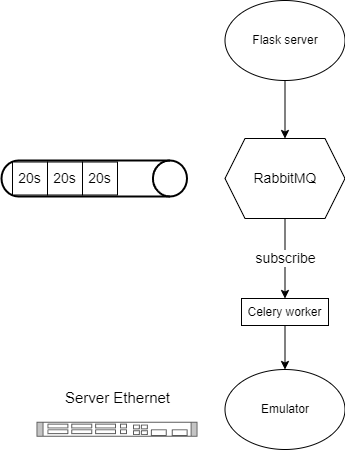
\includegraphics[width=0.45\textwidth, keepaspectratio]{seq.png}
  \end{center}
\end{frame}


\begin{frame}[fragile]
  \frametitle{Ограничения текущей реализации}
  \begin{itemize}
    \item \textbf{Масштабируемость}: Использование одного контейнера для всех эмуляций ограничивает производительность при увеличении количества узлов.
    \item \textbf{Использование ресурсов}: Недостаточная эффективность при многозадачности и ограниченное использование многопроцессорных ресурсов.
    \item \textbf{Сетевые ограничения}: Ограниченная изоляция сетевых стеков между контейнерами, что снижает гибкость и может приводить к конфликтам.
  \end{itemize}
\end{frame}


\begin{frame}
  \frametitle{Постановка задачи}
  \textbf{Целью} является оптимизация и распределённое выполнение сетевых эмуляций в \textbf{Miminet} с использованием Docker для улучшения производительности и масштабируемости системы

  \textbf{Задачи}:
  \begin{itemize}
    \item Разработка архитектуры распределённого выполнения эмуляций с использованием нескольких контейнеров Docker.
    \item Проектирование и внедрение системы управления задачами и балансировки нагрузки для эффективного распределения ресурсов.
    \item Экспериментальное тестирование предложенного подхода на реальных данных и в реальных образовательных условиях.
    \item Валидация результатов с целью подтверждения улучшения производительности и сокращения времени ожидания для студентов.
\end{itemize}
\end{frame}

% Обязательный слайд: четкая формулировка цели данной работы и постановка задачи
% Описание выносимых на защиту результатов, процесса или особенностей их достижения и т.д.
\begin{frame}[fragile]
  \frametitle{Решение проблемы}
  \begin{itemize}
    \item \textbf{Распределение нагрузки}: Использование нескольких Docker-контейнеров для распределения вычислительных ресурсов между эмуляциями, что улучшает масштабируемость системы.
    \item \textbf{Многопроцессорная обработка}: Эффективное использование доступных ядер процессора для параллельной обработки задач, что повышает производительность.
    \item \textbf{Динамическое масштабирование}: Автоматическое добавление контейнеров в зависимости от нагрузки, что позволяет снизить время ожидания студентов и увеличить пропускную способность системы.
  \end{itemize}
\end{frame}


\begin{frame}[fragile]
  \frametitle{Архитектура решения}
  \begin{itemize}
    \item Система основана на распределённых Docker-контейнерах, где каждый контейнер выполняет отдельную симуляцию.
    \item \textbf{Mininet} используется для изоляции эмуляций, что позволяет эффективно управлять ресурсами.
    \item \textbf{Celery + RabbitMQ} используются для распределения задач и балансировки нагрузки между контейнерами.
    \item \textbf{Многопроцессорность}: каждый контейнер может использовать несколько ядер процессора для параллельного выполнения эмуляций.
    \item \textbf{Динамическое масштабирование}: при увеличении нагрузки автоматически добавляются новые контейнеры для улучшения пропускной способности.
  \end{itemize}
\end{frame}


\begin{frame}[fragile]
  \frametitle{Архитектура решения (визуализация)}
  % Insert diagram of the solution architecture here
  \begin{center}
    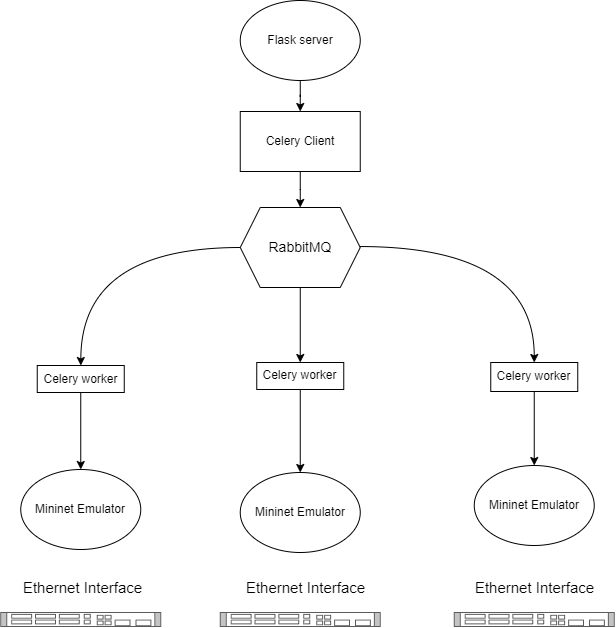
\includegraphics[width=0.58\textwidth]{example.png}
  \end{center}
\end{frame}

\begin{frame}[fragile]
  \frametitle{Проектирование решения}
  \begin{itemize}
    \item Архитектура решения основана на \textbf{распределённом выполнении} эмуляций с использованием нескольких Docker-контейнеров.
    \item Используется \textbf{Celery} и \textbf{RabbitMQ} для распределения задач между рабочими контейнерами.
    \item Количество контейнеров фиксировано, но позволяет выполнять несколько эмуляций одновременно, увеличивая общую пропускную способность.
    \item Улучшена утилизация процессорных ресурсов за счёт балансировки нагрузки между контейнерами.
  \end{itemize}
\end{frame}

\begin{frame}[fragile]
  \frametitle{Экспериментальное тестирование}
  \begin{itemize}
    \item \textbf{Цель}: оценить влияние новой архитектуры на производительность и масштабируемость платформы \textbf{Miminet}.
    \item \textbf{Методика}:
    \begin{itemize}
      \item Сравнение двух версий: одноконтейнерной и многоконтейнерной.
      \item Запуск серии сетевых эмуляций (20 задач подряд).
      \item Время выполнения каждой эмуляции измерялось с помощью встроенного Python-кода:
      \begin{itemize}
        \item \texttt{start = time.time()} до начала задачи;
        \item \texttt{end = time.time()} после завершения;
        \item разница фиксировалась в логах контейнера.
      \end{itemize}
    \end{itemize}

    \item \textbf{Метрики}:
    \begin{itemize}
      \item Время ожидания запуска задачи.
      \item Общее количество параллельно выполняемых задач.
      \item Нагрузка на CPU и использование ресурсов.
    \end{itemize}

    \item \textbf{Результаты}:
    \begin{itemize}
      \item В многоконтейнерной архитектуре удалось запустить до 4 эмуляций одновременно без увеличения времени ожидания.
      \item Среднее время ожидания сократилось с \textbf{~50 секунд} до \textbf{~12 секунд}.
      \item Использование CPU стало более равномерным и эффективным.
    \end{itemize}
  \end{itemize}
\end{frame}

\end{frame}
\begin{frame}[fragile]
  \frametitle{Сравнение производительности}
  \begin{center}
    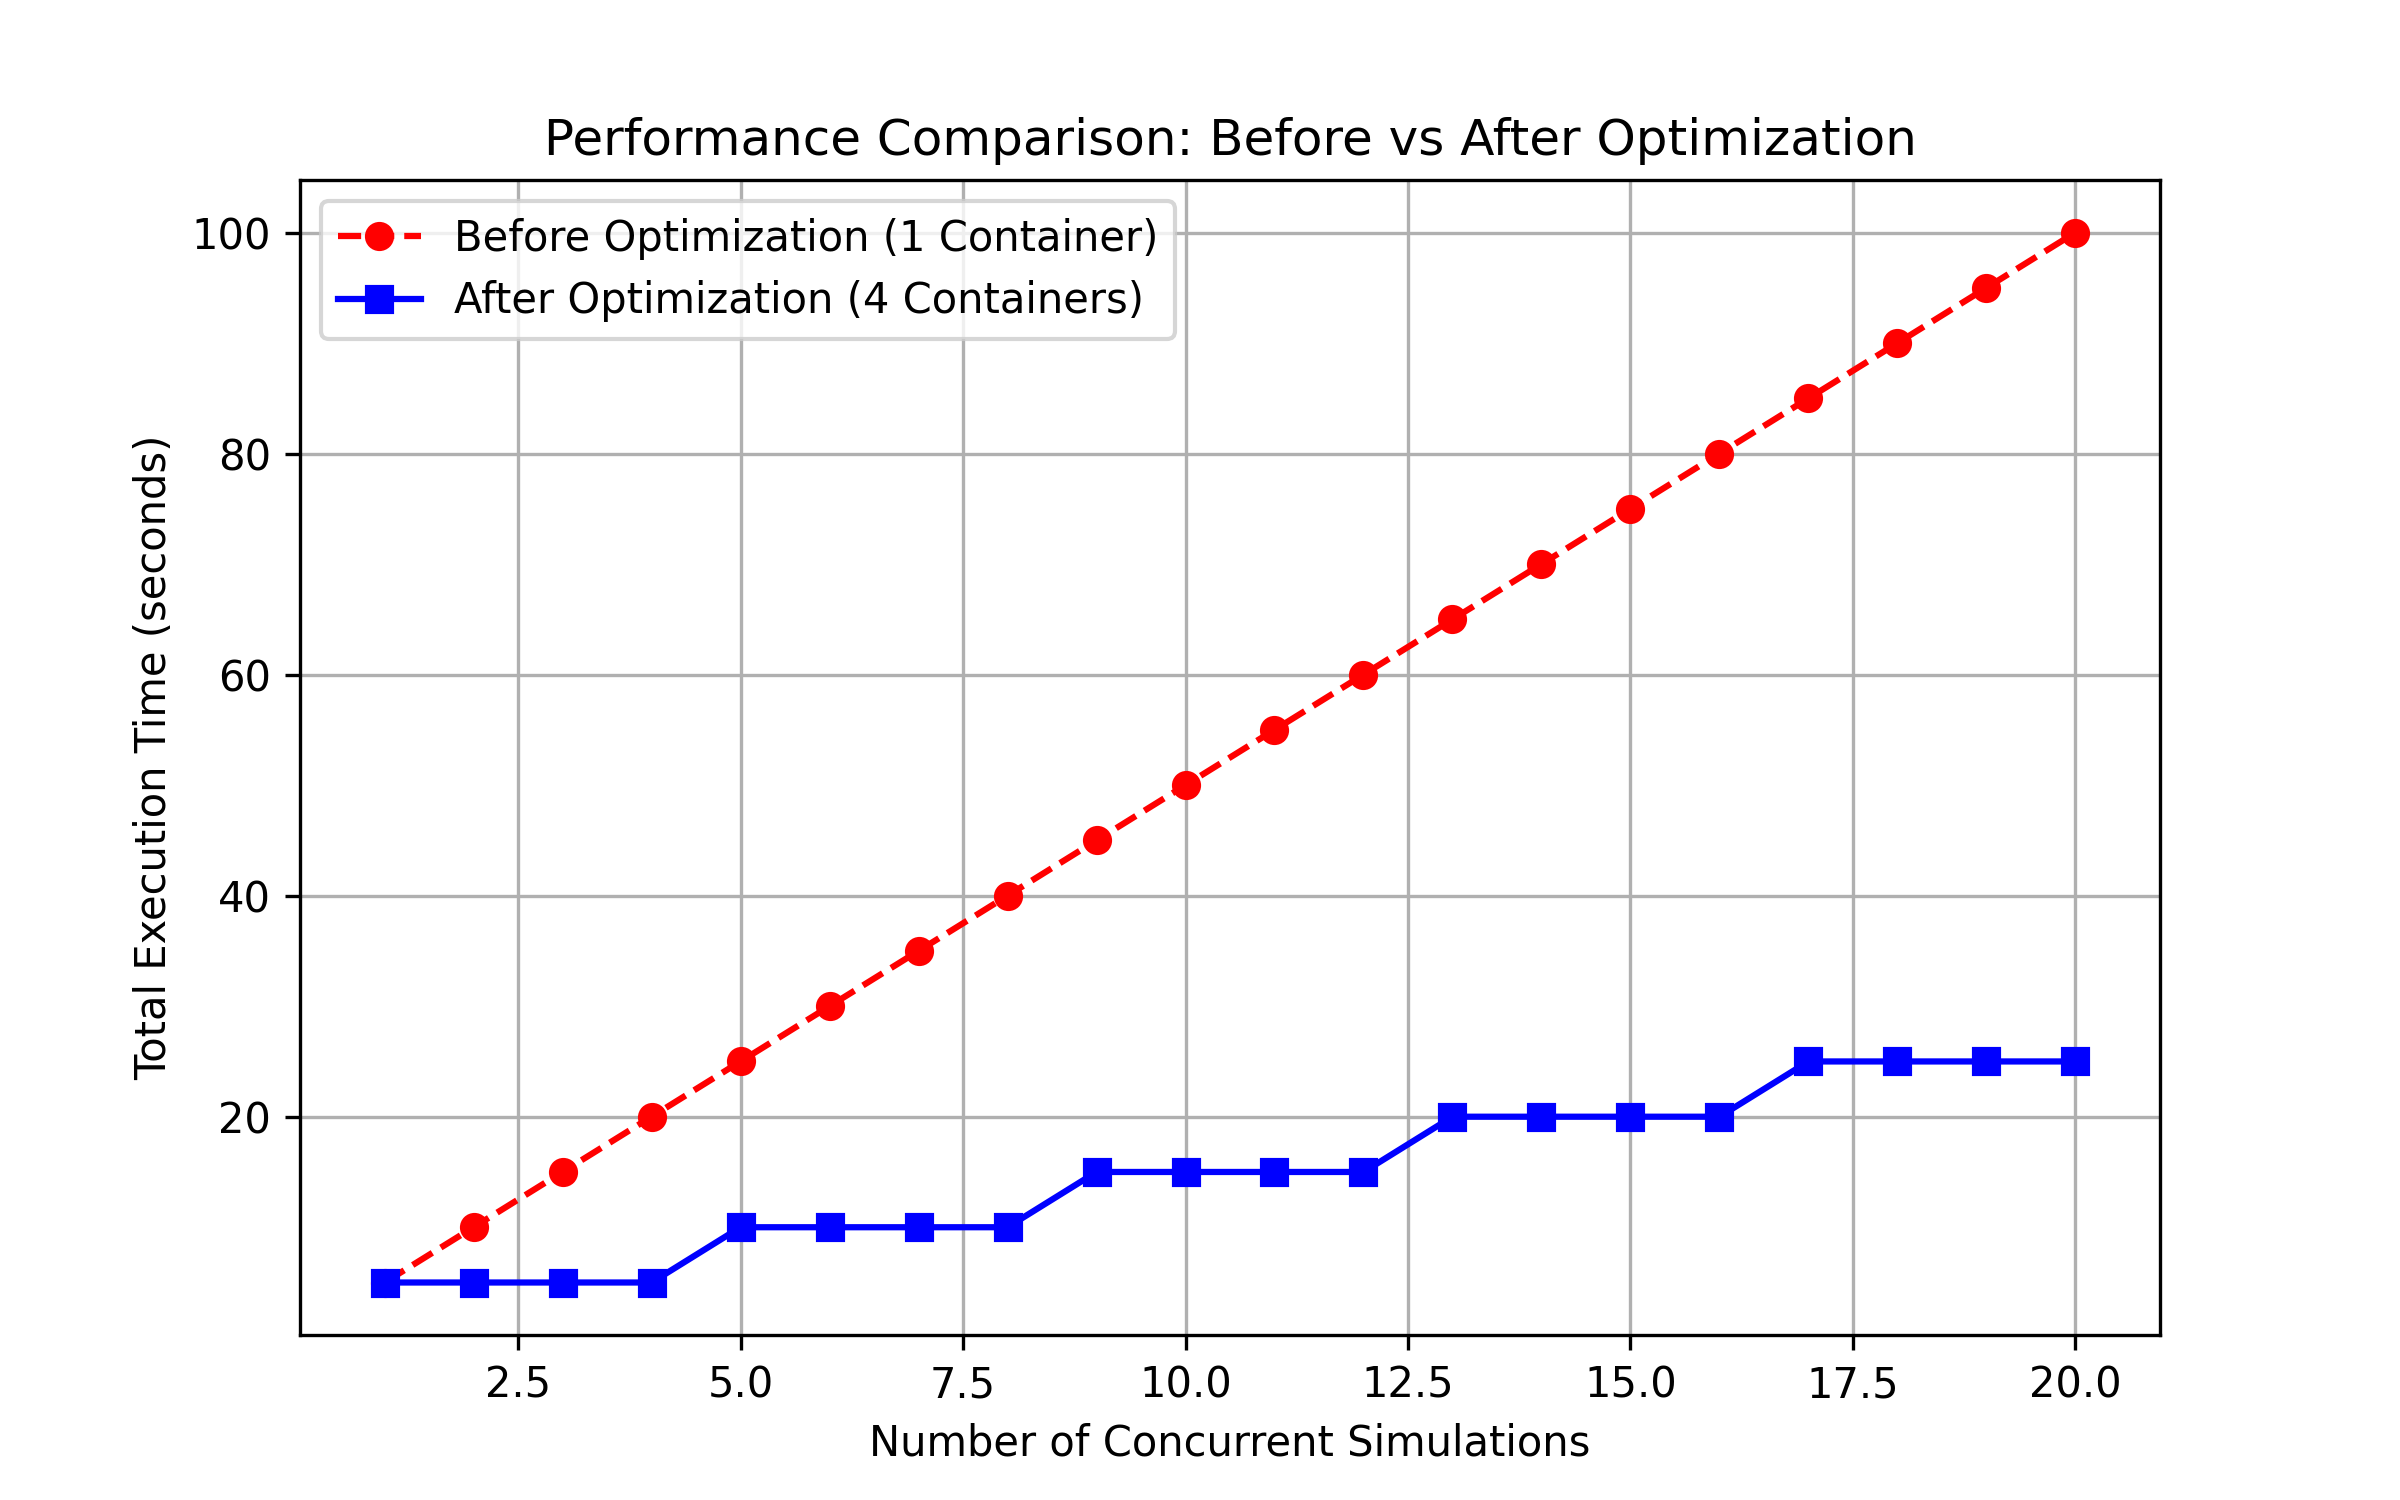
\includegraphics[width=0.8\textwidth]{performance_comparison.png} % Add performance comparison graph
  \end{center}
\end{frame}

% \begin{itemize}
%     \item Сравнение с традиционным методом эмуляции в одном контейнере, без распределённой обработки.
%     \item \textbf{Оценка}:
%     \begin{itemize}
%       \item Влияние на использование процессора (CPU) при увеличении количества эмуляций.
%       \item Влияние на общую пропускную способность системы (количество эмуляций, выполняемых одновременно).
%       \item Потребление памяти и других ресурсов при масштабировании.
%     \end{itemize}
%     \item Результаты:
%     \begin{itemize}
%       \item Уменьшение времени ожидания студентов за счёт параллельного выполнения эмуляций.
%       \item Более равномерное распределение нагрузки и эффективное использование всех вычислительных ресурсов хоста.
%     \end{itemize}
%   \end{itemize}

\begin{frame}[fragile]
  \frametitle{Валидация}
  \begin{itemize}
    \item Проведены тесты на \textbf{производительность и масштабируемость}.
    \item \textbf{Метрики}:
      \begin{itemize}
        \item Общее количество одновременно выполняемых эмуляций увеличено.
        \item Нагрузка на CPU распределяется более равномерно между ядрами, что улучшает общую производительность системы.
        \item Среднее время ожидания запуска эмуляции для студентов сократилось.
      \end{itemize}
    \item \textbf{Вывод}: Оптимизированная архитектура позволяет запускать больше эмуляций параллельно, что снижает нагрузку на сервер и сокращает время ожидания студентов.
  \end{itemize}


\begin{frame}[fragile]
  \frametitle{Выводы}
  \begin{itemize}
    \item Предложенный подход значительно улучшает масштабируемость и производительность \textbf{Miminet}.
    \item Распределение нагрузки между контейнерами позволяет эффективно использовать ресурсы и снизить время ожидания.
    \item Решение делает \textbf{Miminet} более удобным и эффективным инструментом для обучения компьютерным сетям.
    \item В будущем можно расширить функциональность для поддержки ещё более сложных сетевых топологий и сценариев.
  \end{itemize}
\end{frame}
%Идеально, если есть по одному слайду на каждую поставленную задачу


% \begin{frame}[fragile]
%   \frametitle{Архитектура решения}
%   \begin{itemize}
%     \item В реализации интересны архитектура, библиотеки, инструменты
%     \item Не надо добавлять на слайд примеры кода
%   \end{itemize}
%   \begin{center}
%   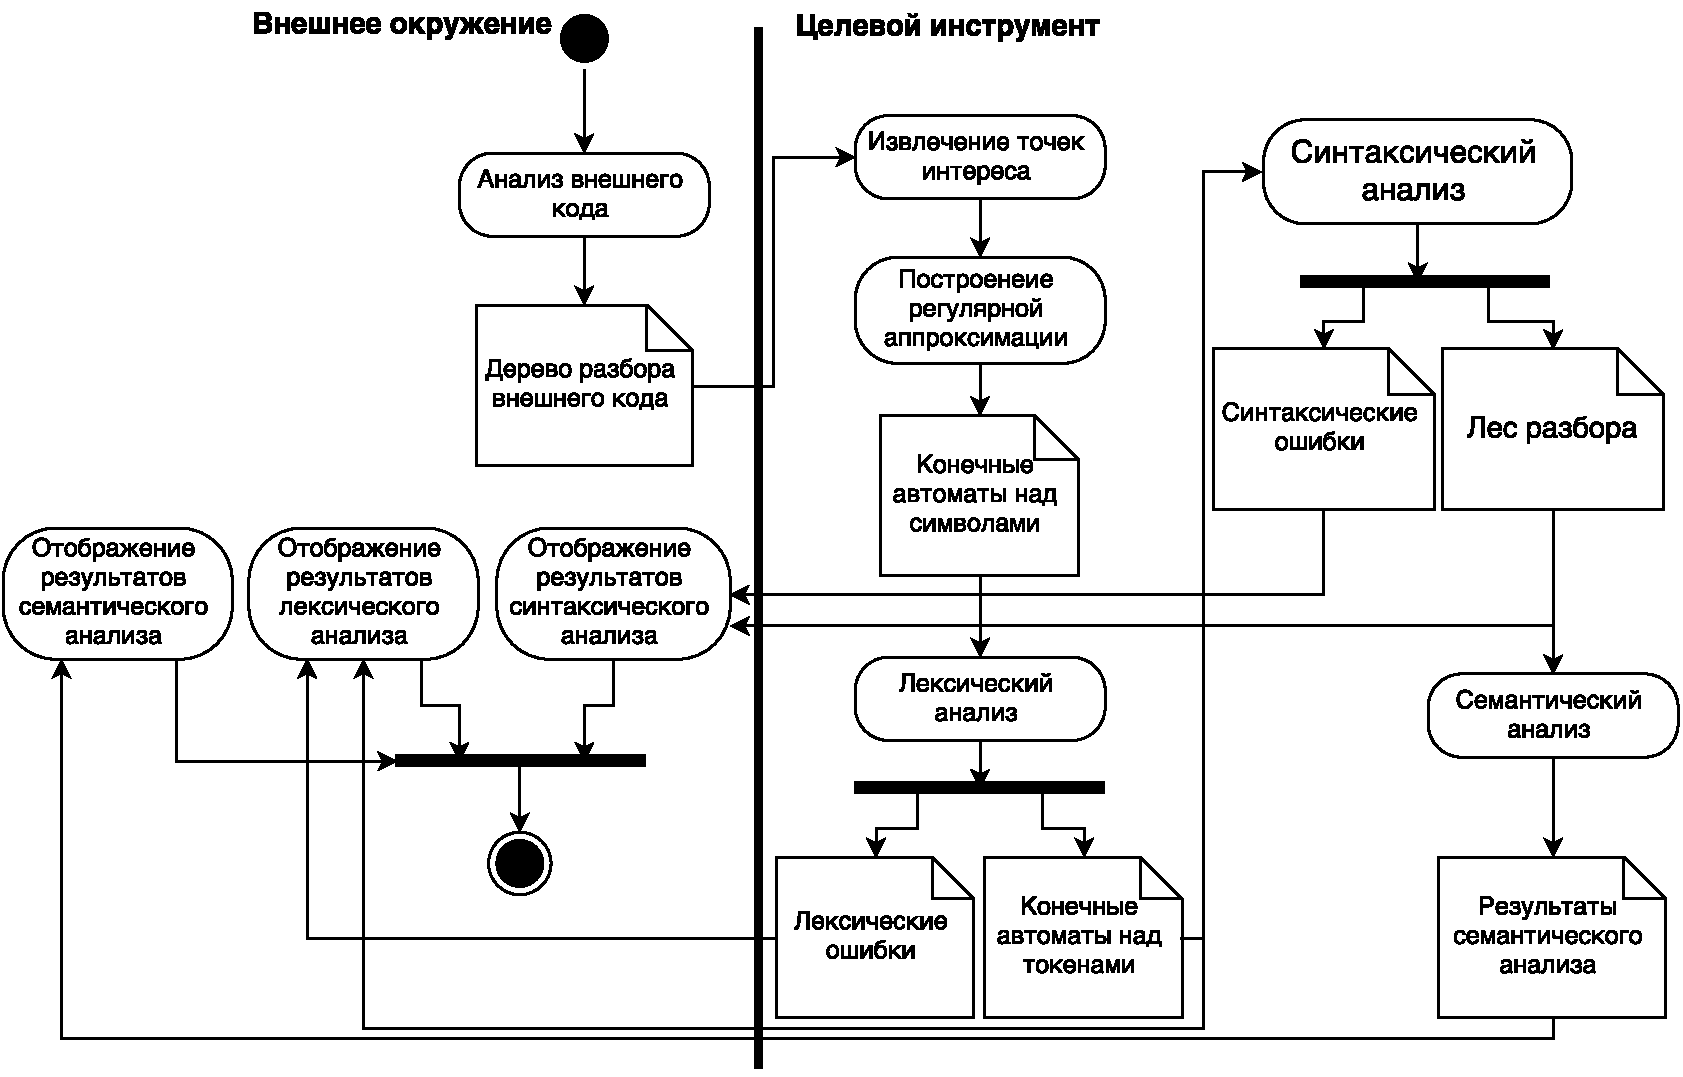
\includegraphics[width=0.8\textwidth]{pictures/Activ_SEL_Processing.pdf}
%   \end{center}
% \end{frame}


% \begin{frame}[t]
%   \frametitle{Результаты экспериментального исследования}
%   \begin{itemize}
%     \item Какие результаты показало экспериментальное исследование
%     \item Желательно привести графики, иллюстрирующие полученные результаты
%     \begin{itemize}
%       \item У иллюстраций должны быть подписи, у графиков~--- легенда, подписи к осям, например:
%     \end{itemize}
%   \end{itemize}
%   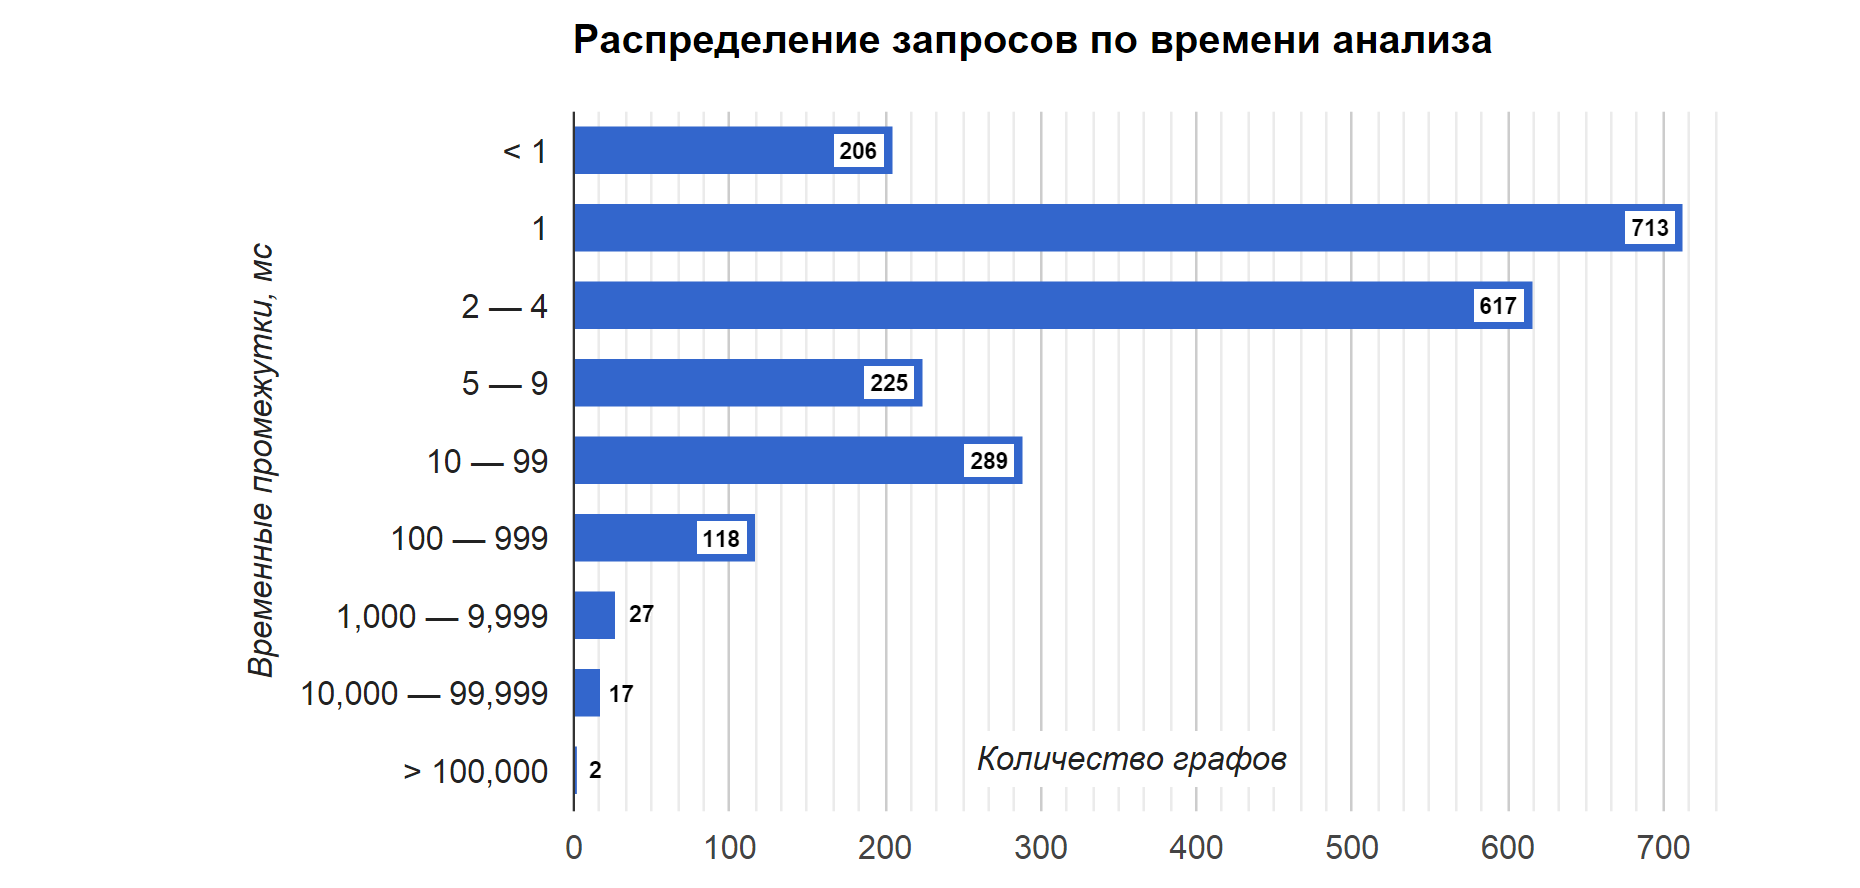
\includegraphics[width=10cm]{pictures/dist.png}
% \end{frame}


% \begin{frame}
%   \frametitle{Результаты}
%   \begin{itemize}
%     \item Практически то же, что и на слайде с постановкой задачи, но в совершенной форме~--- что делал лично автор
%     \item Четкое отделение результатов своей работы (особенно для коллективных работ)
%       \item Формулировать глаголами совершенного вида в прошедшем времени (\enquote{сделано}, \enquote{получено})
%     \item Обсуждение (ограничения, валидность, альтернативы)
%     \item Не нужно слайдов типа \enquote{Все}, \enquote{Вопросы?}, \enquote{Спасибо за внимание}
%   \end{itemize}

%   \begin{itemize}
%     \item Если результаты были представлены на конференции и опубликованы, это желательно указать
%   \end{itemize}
% \end{frame}


\end{document}
